%!TEX program = lualatex
% aspect ratio: 16:9
\documentclass[unicode, 9pt, aspectratio=169]{beamer}
\usepackage{mybeamer}
\usepackage{luatexja-otf}
\usepackage{graphicx}
\usepackage{amsmath}


\title{エネルギー工学I 課題2}
\author{ME2208 \CID{8705}橋 尚太郎}
\institute{明石工業高等専門学校 専攻科 機械・電子システム工学専攻1年}
\date{2023年2月20日}

\begin{document}

\maketitle

\begin{frame}
  \frametitle{発表概要}
  \centering
    \begin{block}{}
      \begin{enumerate}
        \item 取り組んだ課題
        \item 目標
        \item モデル
        \item 計算原理
        \item 実装
        \item 実験結果
        \item 考察・結論
        \item おわりに
      \end{enumerate}
    \end{block}
\end{frame}

\begin{frame}
  \frametitle{取り組んだ課題}
  $\blacksquare$ \underline{対流型サウナ室内の熱気の移動に関するシミュレーション}
  \begin{center}
    \begin{minipage}{.8\linewidth}
        \begin{block}{}
            \centering
            \begin{tabular}{ccc}
                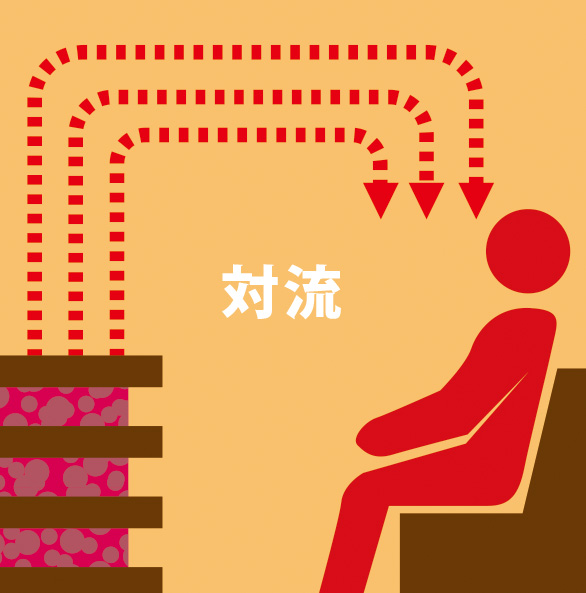
\includegraphics[height=.5\textheight]{img/1.jpg}
                &
                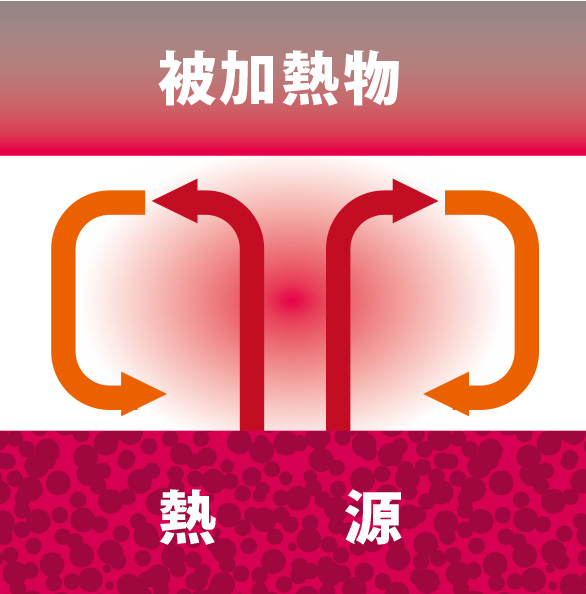
\includegraphics[height=.5\textheight]{img/2.jpg}
                \\ \tiny 対流型サウナの概要: サウナストーンを積んだサウナ & \tiny 対流の仕組み：空気の膨張(上昇)、収縮(下降)。\\
            \end{tabular}
            \\{\tiny [参考] 知っているようで知らないサウナの「熱」の正体 : アットダイム \url{https://dime.jp/genre/1454460/}}
        \end{block}
    \end{minipage}
\end{center}
\vspace{-4truemm}
  \centering
  \begin{minipage}{.5\linewidth}
    \begin{alertblock}{}
        \centering
        \Large \emph{どのように熱が伝わるかが知りたい}
    \end{alertblock}
  \end{minipage}
\end{frame}

\begin{frame}
  \frametitle{目標}
  $\blacksquare$ サウナ室が\textbf{\textcolor{red}{なるべく早く温まる条件}}を求める\\
  $\blacksquare$ サウナ室が\textbf{\textcolor{red}{なるべく快適な条件}}を見つける\\
  \hrulefill\\
  \centering
  \begin{minipage}{.7\linewidth}
    \begin{exampleblock}{方法}
        \centering
        \Large \emph{サウナ室全体が温まるまでの\textbf{\textcolor{red}{所要時間を求める}}}\\
        \Large \emph{窓を付けた場合の温まり方の\textbf{\textcolor{red}{ばらつきを調べる}}}
    \end{exampleblock}
  \end{minipage}  

  \begin{description}
    \item[ex.1] 所要時間の場合\\
  $\to$ サウナ室全体が\textbf{\textcolor{red}{均一に温まった状態}}での実行サイクル数を比較する
    \item[ex.2] ばらつきの場合\\
  $\to$ \textbf{\textcolor{red}{同一実行サイクル数}}でサウナ室の温度分布を比較する
  \end{description}
  \centering
  \begin{minipage}{.5\linewidth}
    \begin{alertblock}{}
        \centering
        \Large \emph{対流型サウナの部屋のモデルを作成する}
    \end{alertblock}
  \end{minipage}
\end{frame}

\begin{frame}
  \frametitle{モデル}
  \vspace{-8pt}

  \hrulefill
  \begin{center}
        \begin{block}{}
          \begin{tabular}{cccc}
            \begin{minipage}{.22\linewidth}
                \begin{figure}
                  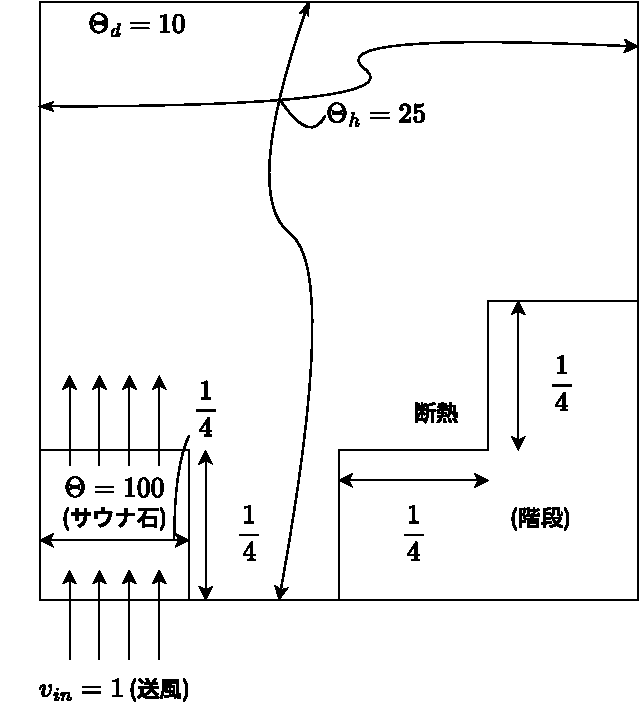
\includegraphics[width=\textwidth]{img/model1.pdf}
                \end{figure}
            \end{minipage}
            &
            \begin{minipage}{.22\linewidth}
                \begin{figure}
                  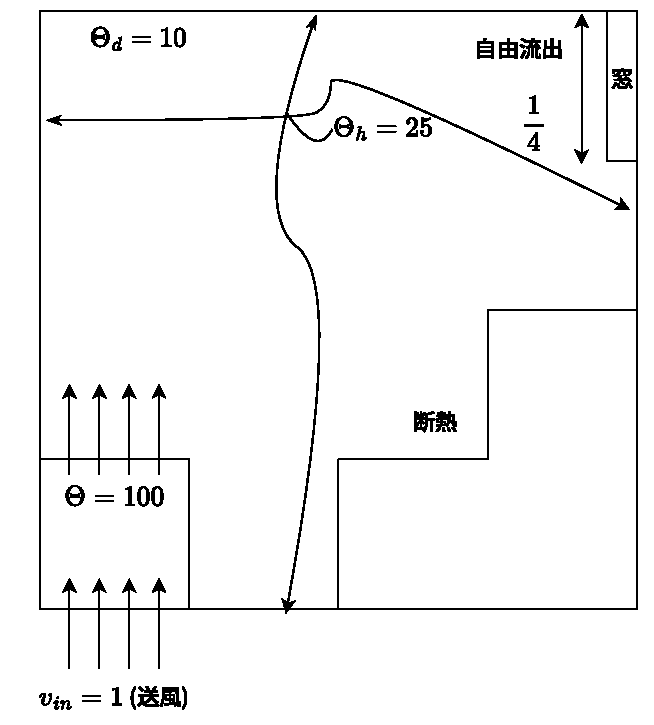
\includegraphics[width=\textwidth]{img/model2.pdf}
                \end{figure}
            \end{minipage}
            &
            \begin{minipage}{.22\linewidth}
                \begin{figure}
                  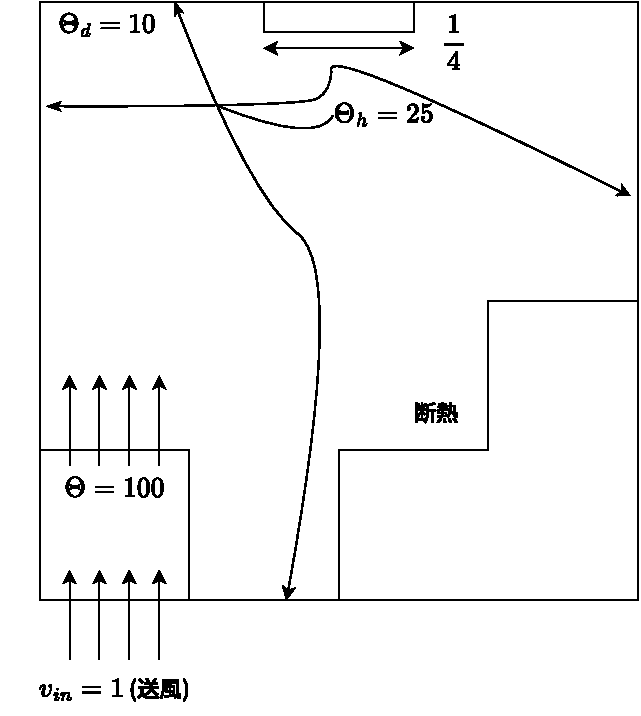
\includegraphics[width=\textwidth]{img/model3.pdf}
                \end{figure}
            \end{minipage}
            &
            \begin{minipage}{.22\linewidth}
                \begin{figure}
                  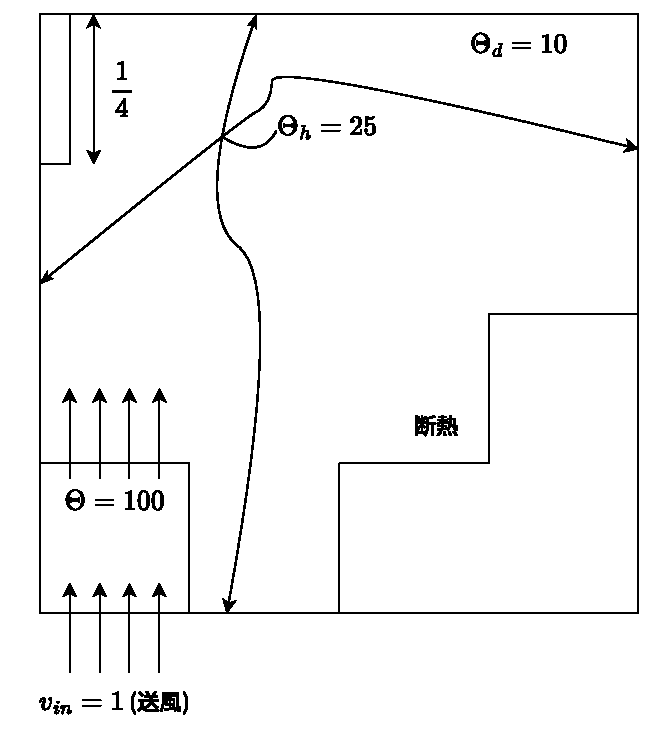
\includegraphics[width=\textwidth]{img/model4.pdf}
                \end{figure}
            \end{minipage}
          \end{tabular}
        \end{block}
\end{center}

\centering
\begin{minipage}{.8\linewidth}
\centering
\vspace{-3.5truemm}
\begin{exampleblock}{境界条件の設定}
  \begin{description}
    \item[サウナ石] $P=0,  \Theta = 100$
    \item[(窓)自由流出] $\partial P/\partial X = \partial U/\partial X = \partial \Theta_h/\partial X = 0,  V = 0$ (左右面の場合)
    \item[断熱条件] $\partial \Theta/\partial X = 0, (\Theta/\partial Y = 0)$ 
  \end{description}
\end{exampleblock}
\end{minipage}

\end{frame}

\begin{frame}
  \frametitle{計算原理}
  \centering
  \begin{minipage}{.8\linewidth}
    \vspace{-8truemm}
    \begin{block}{所要時間tを求める式}
      \vspace{-5truemm}
      \begin{align}
        Re &= u_0x_0/\nu, (\nu ：動粘性係数(物性値))\\
        t_0 &= x_0/u_0 \\
        t &= t_0T
      \end{align}
    \end{block}
    \begin{exampleblock}{既知の値}
      \centering
      $Re$：パラメータファイルで指定, $x_0$：1としている, \\$T$：時間の刻み幅(DT)$\times$ステップ数(NCYCLE)
    \end{exampleblock}
    \begin{alertblock}{}
      \centering
      \Large \emph{\textbf{\textcolor{red}{流体の物性値が分かれば\\レイノルズ数と無次元化の関係式から所要時間を求めることができる!!}}}
    \end{alertblock}
  \end{minipage}
\end{frame}

\begin{frame}
  \frametitle{実装}
  $\blacksquare$ 実行環境：Visual Studio Code\\
  $\blacksquare$ コンパイラ：MinGW-w64 GCC (Minimalist GNU for Windows) クロスコンパイラ\\
  $\blacksquare$ OS：Windows 10 Pro, メモリ：8GB, SSD：256GB
  \vspace{-8pt}

  \hrulefill
  \begin{center}
          \begin{tabular}{cccc}
            \begin{minipage}{.22\linewidth}
              cinit関数
                \begin{figure}
                  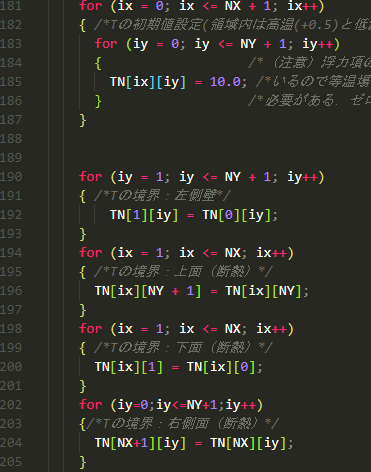
\includegraphics[width=\textwidth]{img/jouken1_1_cinit.png}
                \end{figure}
            \end{minipage}
            &
            \begin{minipage}{.22\linewidth}
              階段部の速度の境界条件
                \begin{figure}
                  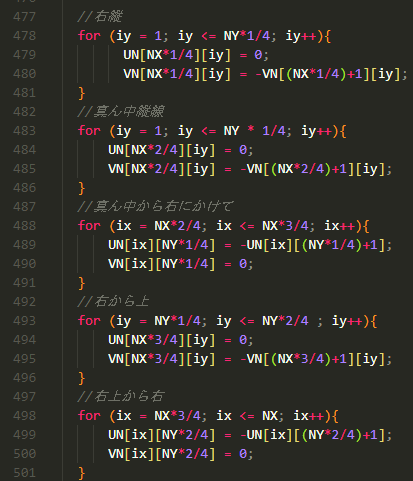
\includegraphics[width=\textwidth]{img/jouken1_2_kaidansokudo.png}
                \end{figure}
            \end{minipage}
            &
            \begin{minipage}{.22\linewidth}
              断熱条件
                \begin{figure}
                  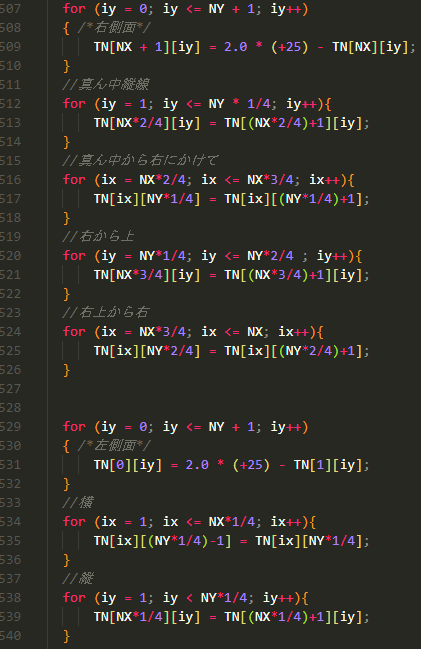
\includegraphics[width=\textwidth]{img/jouken1_3_dannnetsu.png}
                \end{figure}
            \end{minipage}
            &
            \begin{minipage}{.22\linewidth}
              熱流の吹き出し口
                \begin{figure}
                  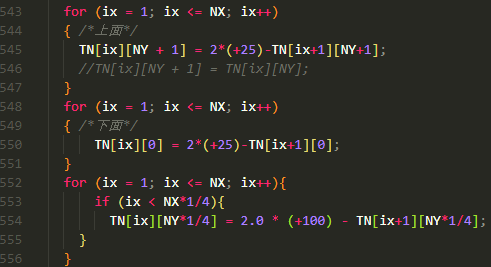
\includegraphics[width=\textwidth]{img/jouken1_4_fukidashi.png}
                \end{figure}
            \end{minipage}
          \end{tabular}
\end{center}
\end{frame}

\begin{frame}
  \frametitle{実験結果1/3 (動画)}
\end{frame}

\begin{frame}
  \frametitle{実験結果2/3}
  $\blacksquare$ 所要時間に関して(目標との照合1/2)
  \vspace{-8pt}

  \hrulefill
  \begin{center}
        \begin{block}{}
          \begin{tabular}{cccc}
            \begin{minipage}{.22\linewidth}
                \begin{figure}
                  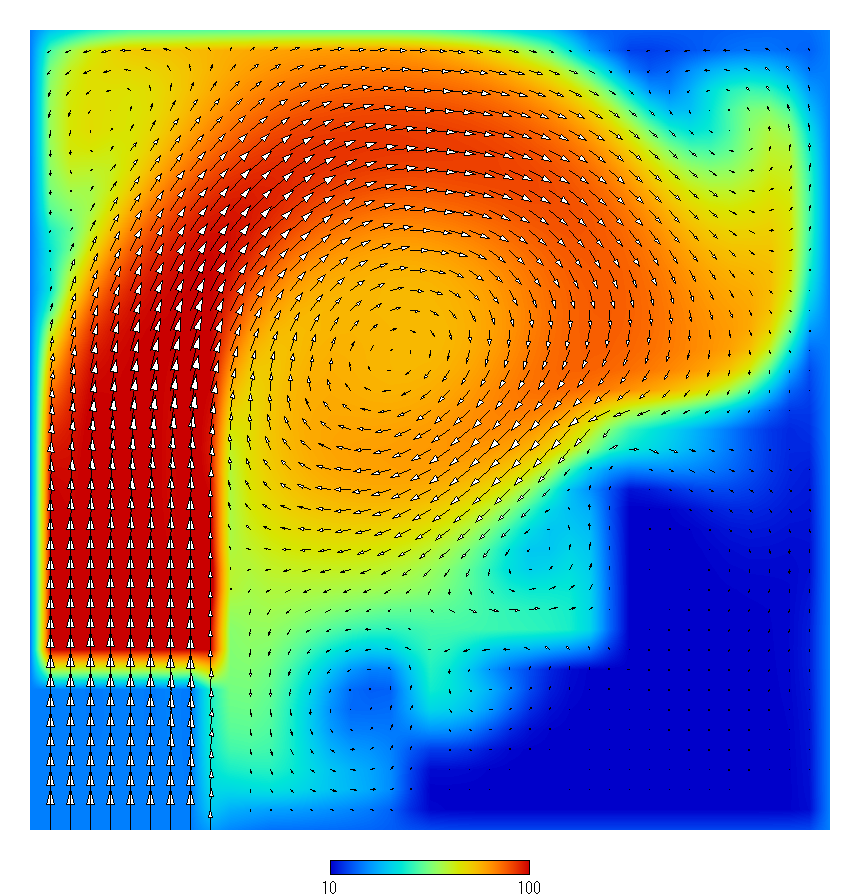
\includegraphics[width=\textwidth]{img/kadai2_55000.png}
                \end{figure}
            \end{minipage}
            &
            \begin{minipage}{.22\linewidth}
                \begin{figure}
                  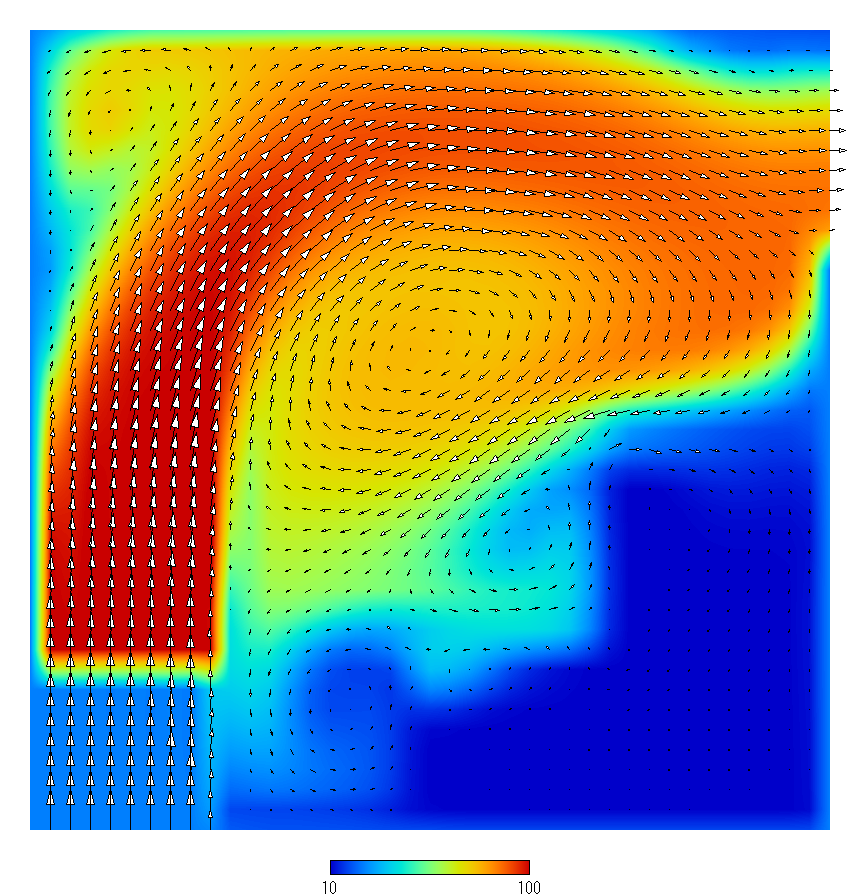
\includegraphics[width=\textwidth]{img/kadai2_45000.png}
                \end{figure}
            \end{minipage}
            &
            \begin{minipage}{.22\linewidth}
                \begin{figure}
                  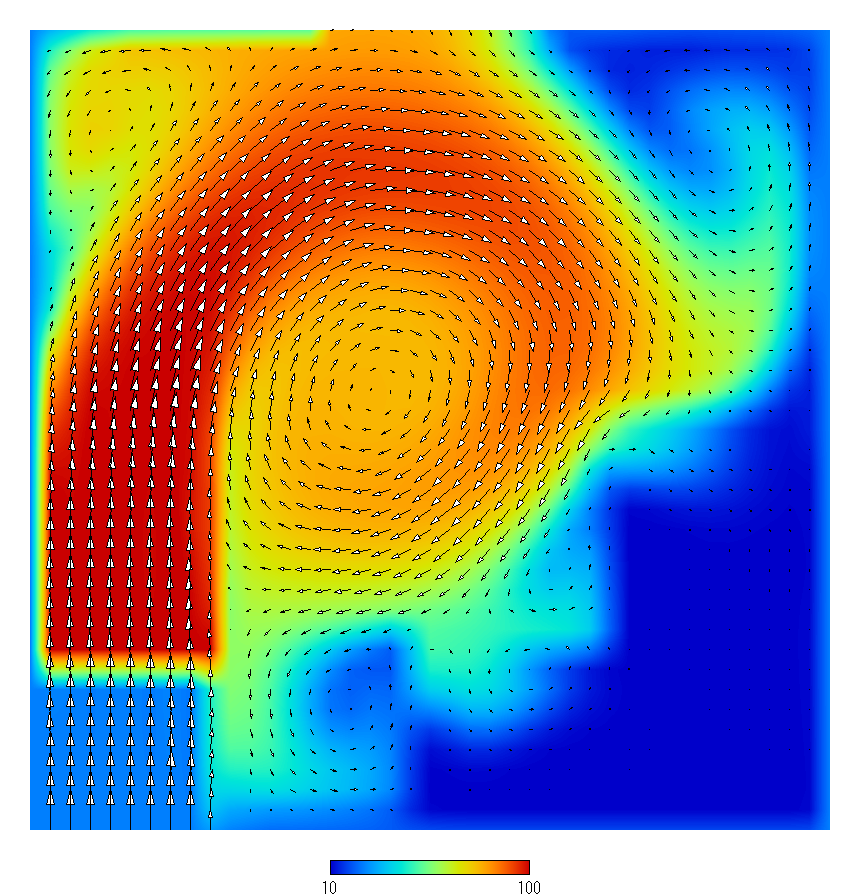
\includegraphics[width=\textwidth]{img/kadai2_50000.png}
                \end{figure}
            \end{minipage}
            &
            \begin{minipage}{.22\linewidth}
                \begin{figure}
                  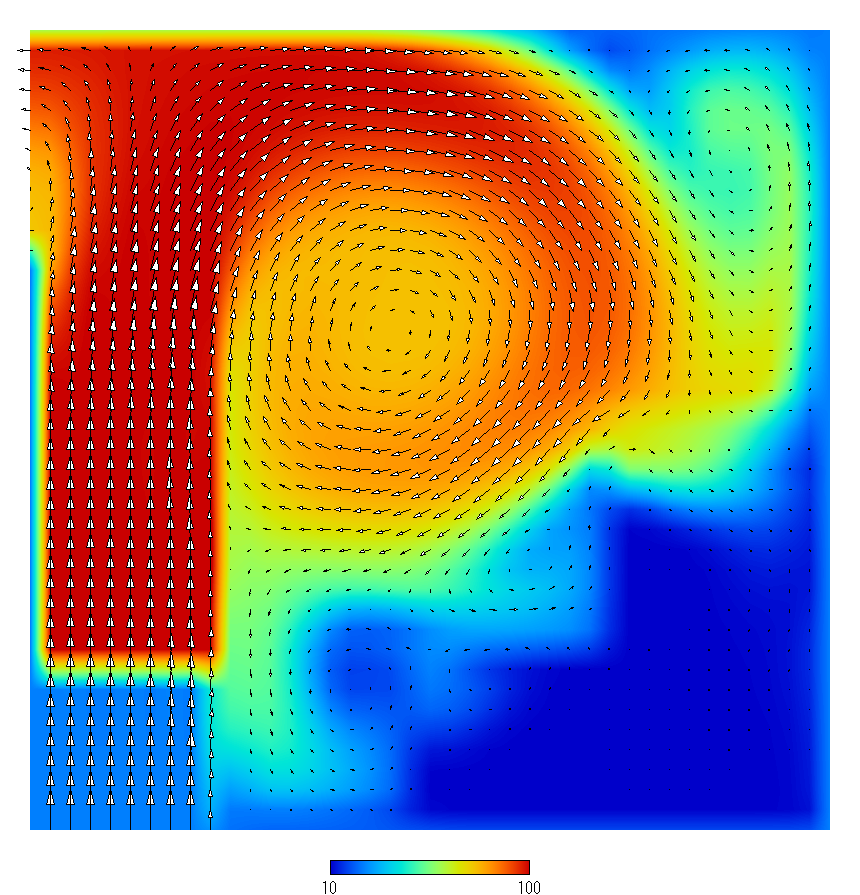
\includegraphics[width=\textwidth]{img/kadai2_65000.png}
                \end{figure}
            \end{minipage}\\
            \tiny 窓無し NCYCLE=55000, (3.4時間) & \tiny 右壁面に窓 NCYCLE=45000, \textbf{\textcolor{red}{(2.8時間)}}& \tiny 上面に窓 NCYCLE=50000, (3.1時間)& \tiny 左壁面に窓 NCYCLE=65000, (3.9時間)
          \end{tabular}
        \end{block}
        \begin{minipage}{.8\linewidth}
          \begin{alertblock}{}
            \centering
            \Large \emph{\textbf{\textcolor{red}{右壁面に窓があると部屋が早く温まる!!\\その後NCYCLE=100000(6.1時間)までシミュレーションを実行}}}
          \end{alertblock}
        \end{minipage}
\end{center}
\end{frame}

\begin{frame}
  \frametitle{実験結果3/3}
  $\blacksquare$ 温度分布のばらつきについて(目標との照合2/2)
  \vspace{-8pt}

  \hrulefill
  \begin{center}
        \begin{block}{}
          \begin{tabular}{cccc}
            \begin{minipage}{.22\linewidth}
                \begin{figure}
                  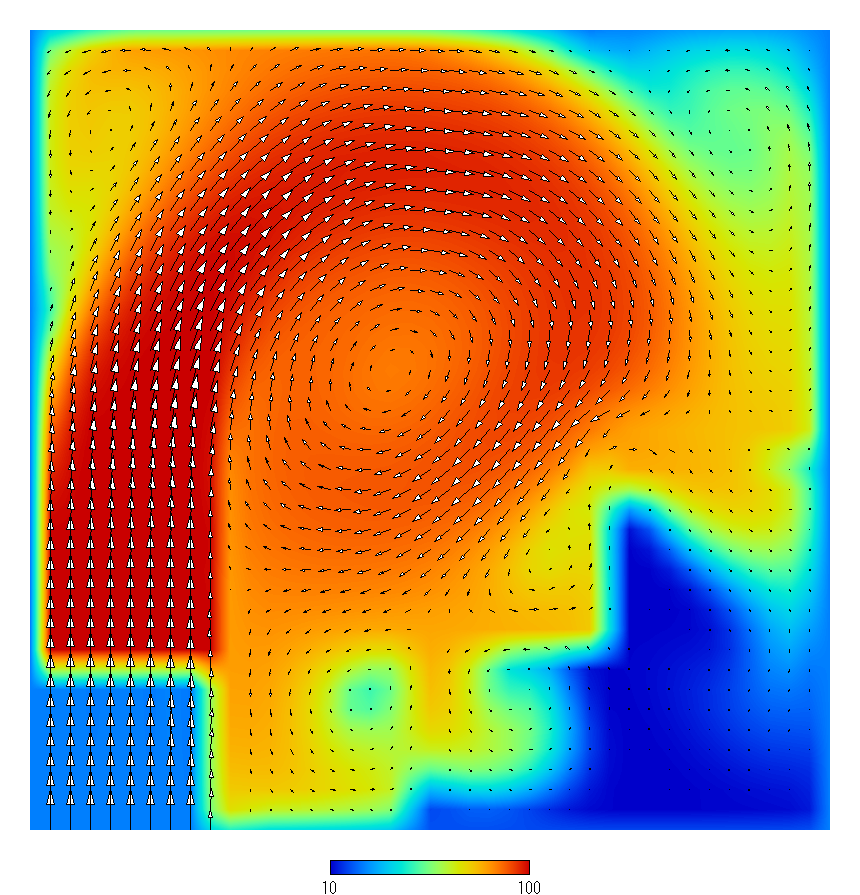
\includegraphics[width=\textwidth]{img/kadai2_1_100000.png}
                \end{figure}
            \end{minipage}
            &
            \begin{minipage}{.22\linewidth}
                \begin{figure}
                  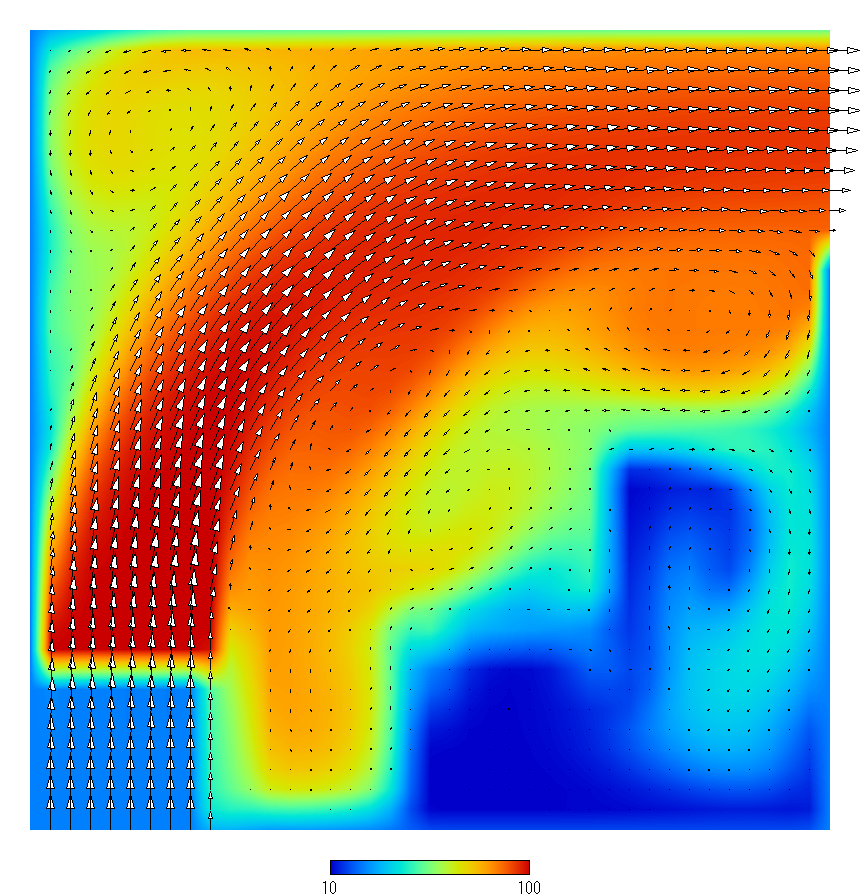
\includegraphics[width=\textwidth]{img/kadai2_2_100000.png}
                \end{figure}
            \end{minipage}
            &
            \begin{minipage}{.22\linewidth}
                \begin{figure}
                  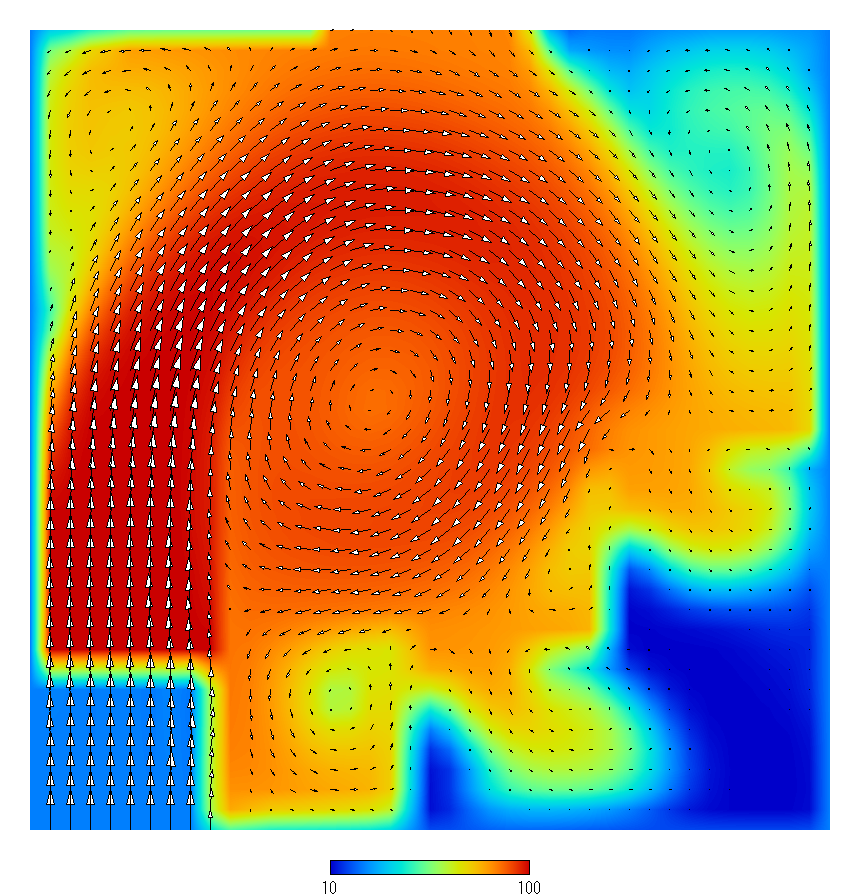
\includegraphics[width=\textwidth]{img/kadai2_3_100000.png}
                \end{figure}
            \end{minipage}
            &
            \begin{minipage}{.22\linewidth}
                \begin{figure}
                  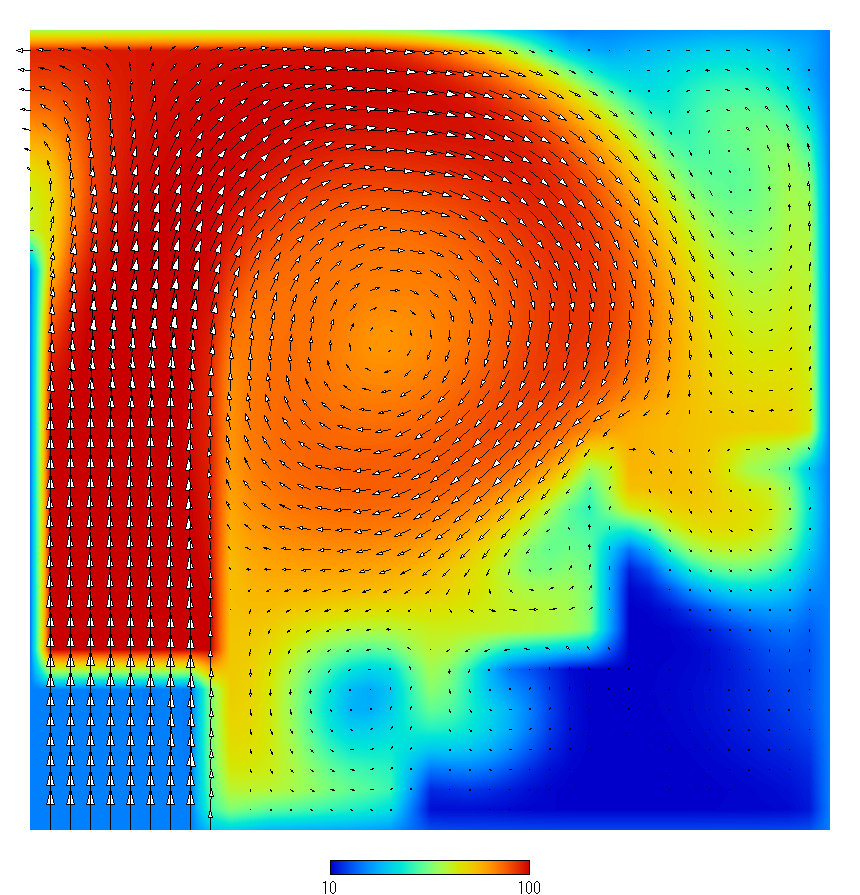
\includegraphics[width=\textwidth]{img/kadai2_4_100000.png}
                \end{figure}
            \end{minipage}\\
            \tiny 窓無し 基準 & \tiny 右壁面に窓 \textbf{\textcolor{red}{(熱気が上に逃げる)}}& \tiny 上面に窓  \textbf{\textcolor{red}{(均等に温度が分布)}} & \tiny ばらつきあり 
          \end{tabular}
        \end{block}
        \begin{minipage}{.8\linewidth}
          \begin{alertblock}{}
            \centering
            \Large \emph{\textbf{\textcolor{red}{上面に窓を付けても熱気の流れに変化がなく温度が均等に分布}}}\\
            \Large \emph{\textbf{\textcolor{red}{右壁面に窓がある場合温まりやすく冷めやすい!!}}}
          \end{alertblock}
        \end{minipage}
\end{center}
\end{frame}



\begin{frame}
  \frametitle{考察・結論}
  \begin{description}[目的]
    \item[考察] 早く温まる場合・温度分布のばらつきが少ない場合が存在$\to$\textbf{\textcolor{red}{窓の取り付け位置を組み合わせる}}
    \item[結論] 窓を複数個所に設置して時間ごとに換気のタイミングを制御する仕組み
  \end{description}
  \begin{center}
    \vspace{-8pt}

    \hrulefill

    \begin{tabular}{cc}
        \begin{minipage}{.5\linewidth}
            部屋全体が温まるまでは右側窓を換気(上面窓はOFF)
            \begin{figure}
              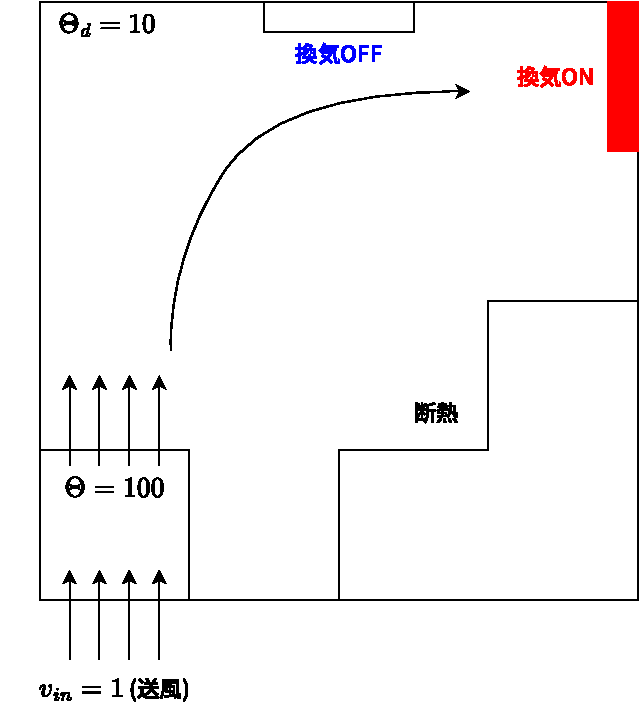
\includegraphics[width=.6\textwidth]{img/model5.pdf}
            \end{figure}
        \end{minipage}
        &
        \begin{minipage}{.5\linewidth}
            部屋全体が温まると上面窓を換気(右側窓はOFF)
            \begin{figure}
              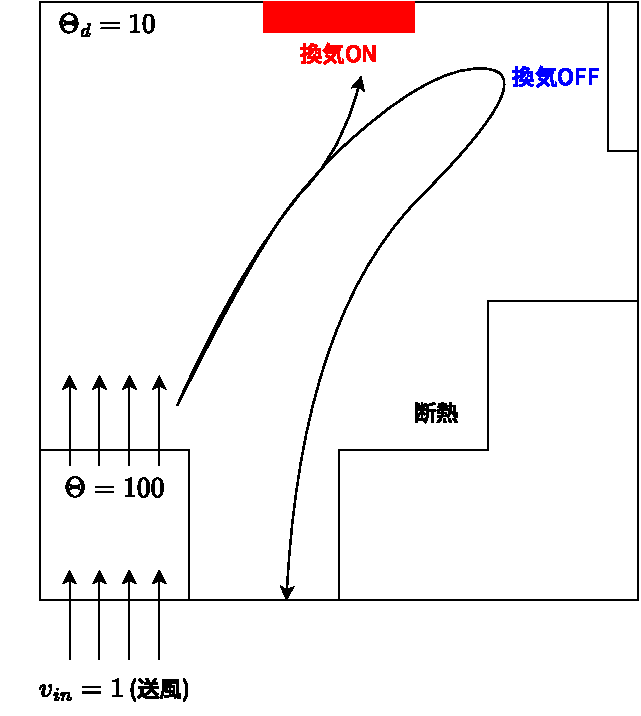
\includegraphics[width=.6\textwidth]{img/model6.pdf}
            \end{figure}
        \end{minipage}
    \end{tabular}
\end{center}
\end{frame}


\begin{frame}
  \frametitle{おわりに}
  $\blacksquare$ サウナ室が\textbf{\textcolor{red}{なるべく早く温まる条件}}
  $\to$ 右壁面に窓を付ける\\
  $\blacksquare$ サウナ室が\textbf{\textcolor{red}{なるべく快適な条件}}
  $\to$ 上面の窓と右壁面の窓の換気制御\\

    \hrulefill

    \begin{tabular}{cc}
        \begin{minipage}{.5\linewidth}
          $\blacksquare$ 改善点
          \begin{block}{python を使って分かりやすく}
            \begin{description}[]
              \item[ex.1] ファイルの出力 $\to$ グラフ化 $\to$ 画像出力 \\$\to$ 動画出力$\to$これらの処理を自動で行いたい
              \item[ex.2] Pythonは可視化ツールが豊富で数値解析に便利 
            \end{description}
            {\tiny [参考] 2次元キャピティ流れをPythonで実装する  \url{https://takun-physics.net/10217/}}
          \end{block}
        \end{minipage}
        &
        \begin{minipage}{.5\linewidth}
          \begin{figure}
            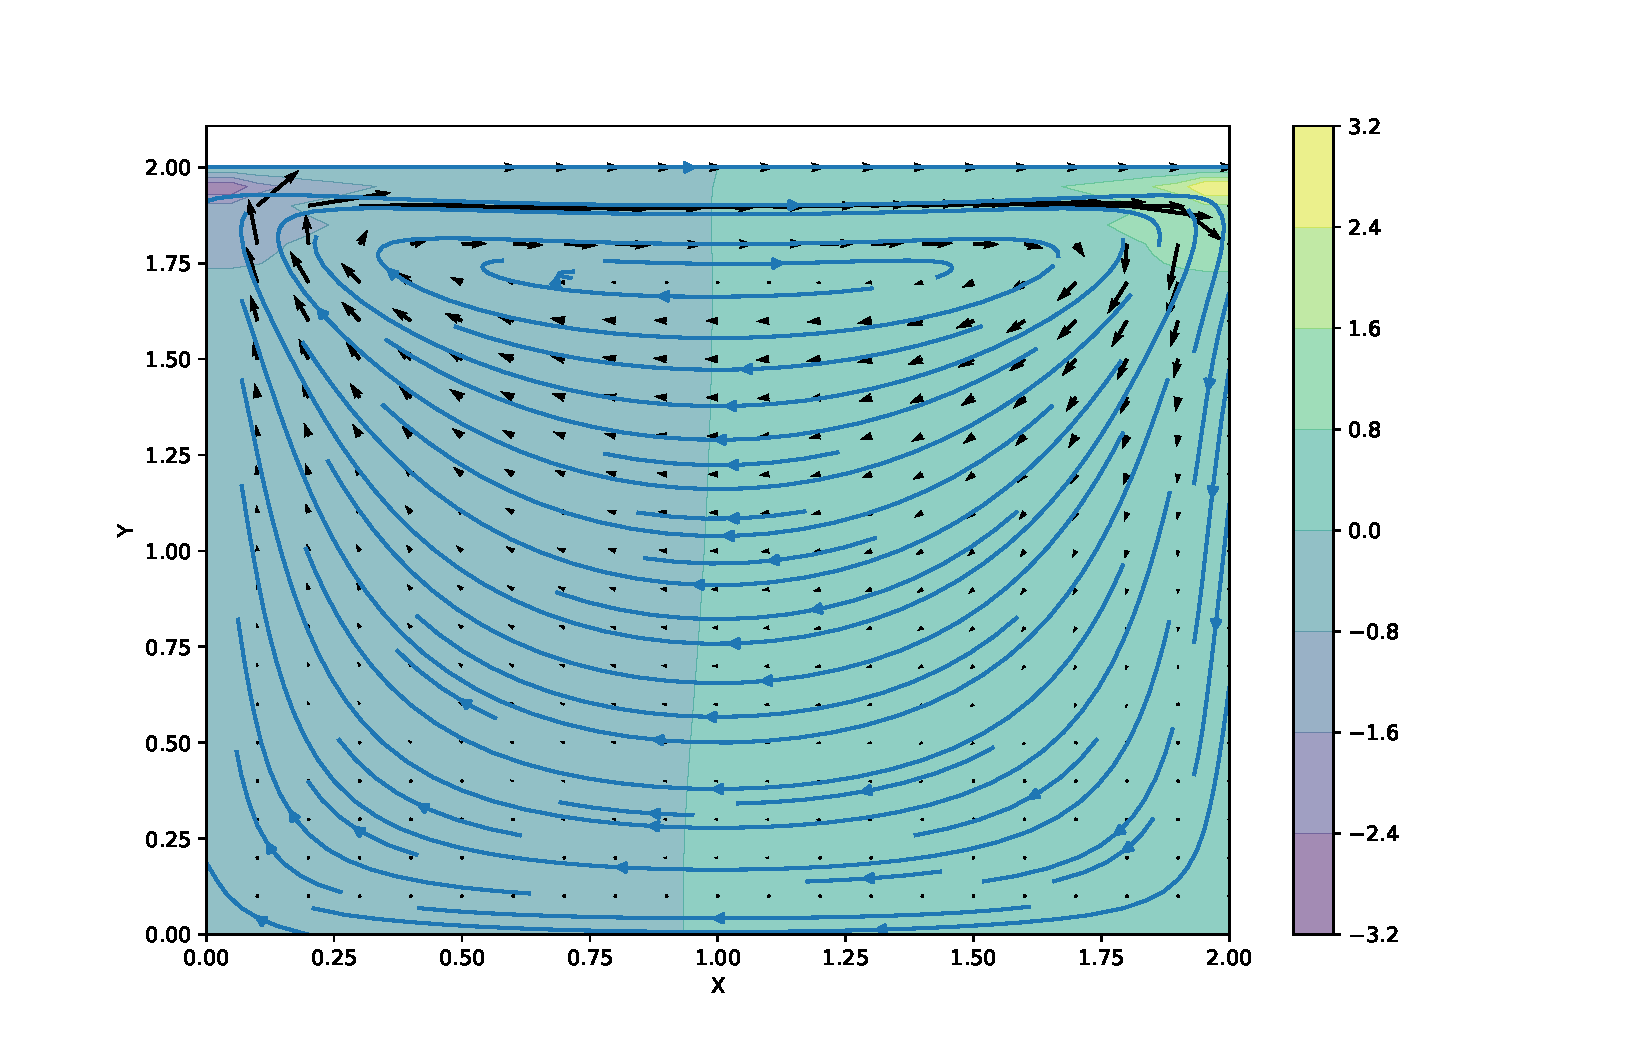
\includegraphics[width=\textwidth]{img/python_sim.pdf}
          \end{figure}
        \end{minipage}
    \end{tabular}
\end{frame}

\end{document}